\DeclareRobustCommand{\dlo}[1]{}
\DeclareRobustCommand{\wen}[1]{#1}

\published{Geophysics, 86, no. 5, V419–V429, (2021)}

\title{5D de-aliased seismic data interpolation using non-stationary prediction error filter}

\author{Yangkang Chen\footnotemark[1], Sergey Fomel\footnotemark[2], Hang Wang\footnotemark[1], and Shaohuan Zu\footnotemark[3]}

\renewcommand{\thefootnote}{\fnsymbol{footnote}}


\ms{GEO-2021} 

\address{
\footnotemark[1]
School of Earth Sciences\\
Zhejiang University\\
Hangzhou, Zhejiang Province, China, 310027\\
chenyk2016@gmail.com \\
\footnotemark[2]Bureau of Economic Geology \\
John A. and Katherine G. Jackson School of Geosciences \\
The University of Texas at Austin \\
University Station, Box X \\
Austin, TX 78713-8924 \\
sergey.fomel@beg.utexas.edu\\
\footnotemark[3] College of Geophysics\\
Chengdu University of Technology \\
Dongsanlu, Erxianqiao, Chengdu 610059, Sichuan, China\\
Corresponding author: Yangkang Chen, chenyk2016@gmail.com
}

\lefthead{Chen et al., 2021}
\righthead{5D NPEF}

\maketitle

\begin{abstract}
The prediction error filter (PEF) assumes that the seismic data can be destructed to zero by applying a convolutional operation between the target data and prediction filter in either time-space or frequency-space domain. Here, we extend the commonly known PEF in 2D or 3D problems to its 5D version. To handle the non-stationary property of the seismic data, we formulate the PEF in a non-stationary way, which is called the non-stationary prediction error filter (NPEF). In the NPEF, the coefficients of a fixed-size PEF vary across the whole seismic data. In NPEF, we aim at solving a highly ill-posed inverse problem via the computationally efficient iterative shaping regularization. The NPEF can be used to denoise multi-dimensional seismic data, and more importantly, to restore the highly incomplete aliased 5D seismic data. We compare the proposed NPEF method with the state-of-the-art rank-reduction method for the 5D seismic data interpolation in cases of irregularly and regularly missing traces via several synthetic and real seismic data. Results show that although the proposed NPEF method is less effective than the rank-reduction method in interpolating irregularly missing traces especially in the case of low signal to noise ratio (S/N), it outperforms the rank-reduction method in interpolating aliased 5D dataset with regularly missing traces.
\end{abstract}

%\section{Keywords}
%key1,key2,key3

\section{Introduction}
\wen{The prediction}\dlo{Prediction} error filter (PEF) is a classic algorithm that has been widely used in many geophysical estimation problems \cite[]{peacock1969predictive,ott1972kalman,kumaresan1983zeros,wanghang2021geo}.  \cite{sacchi2009adaptive} apply the PEF to attenuate random noise in seismic data assuming that the local seismic data can be modeled by a superposition of several planar waves. \cite{haleseamless} proposes a local PEF to filter seismic images. PEF can be implemented in either time-space domain or frequency-space domain. The time-space PEF can better deal with the aliasing issue of the regularly missing seismic traces \cite[]{abma1995}. The frequency-space PEF can be understood \dlo{as }as solving a Z-transform polynomial equation, the roots of which correspond to different plane-wave components \cite[]{canales1984,yangkang20141}. 

\dlo{PEF can be closely related with the well-known plane-wave destruction}\wen{The PEF is closely related to the plane-wave destruction} (PWD) filter \cite[]{fomel2002pwd}, which has been widely used to estimate the local slope of a seismic dataset. The PWD filter is normally estimated in the time-space domain, where the plane-wave differential equation is discretized by a finite-difference method. The discretization connects the local slope with the seismic data through a non-linear relation. Each finite-difference stencil is a non-linear function of the non-stationary local slope. The non-linear relation between local slope and seismic data is then linearized for estimating the local slope by linear inversion. Given a local slope map, the discretized PWD filter has the exact form as a PEF, where the coefficients of a PEF are directly related to the local slope. Thus, both time-space and frequency-space PEFs can be thought of predicting the plane waves. 

\wen{Seismic data interpolation is an important application of PEFs.} \cite{spitz1991} develops the frequency-space PEF to interpolate aliased seismic data, where the coefficients of the PEF are estimated from the less-aliased low-frequency data and then applied to aliased high-frequency data for the interpolation. \cite{claerbout1992pvi} extends the Spitz's method to the time-space PEF to interpolate aliased seismic data. \cite{porsani1999seismic} developed the half-step PEF to interpolate seismic data with much greater computational efficiency. When the PEF is applied locally, the PEF can handle the non-stationary seismic data. The very early application of the non-stationary prediction error filter (NPEF) to seismic trace interpolation was introduced in \cite{crawley2000seismic}. Crawley's strategy for NPEF was based on\dlo{ the} local patches, where the seismic data are assumed to be locally stationary and thus can be interpolated using the classic PEF. To avoid the abrupt change on the edge of each patch after interpolation, the patches are smoothed around the edges. \cite{curry2006interpolating} applies the NPEF to interpolate diffracted multiples. Most NPEF applications are based on segmented local windows, which rely on carefully chosen parameters like window size, tapering width, and PEF parameters inside the local windows. 

\cite{fomel2002pwd} designs a NPEF framework that does not depend on \dlo{the }local windows. Instead, the NPEF is estimated completely via least-squares inversion. In \cite{fomel2002pwd}, the local slope that is directly related with the NPEF coefficients is estimated by shaping regularization with local smoothness constraint.  The window-related parameters are substituted and controlled by the smoothing radius during the inversion.  Based on a similar strategy, \cite{liuyang2011rna} develop the NPEF method for interpolating 2D/3D seismic data, where the NPEF coefficients are estimated by solving a least-squares inverse problem. In addition to the NPEF in the time-space domain, its frequency-space domain counterpart was developed in \cite{guochang2012} and was called the regularized non-stationary autoregression. However, compared with the frequency-space domain NPEF, the time-space domain approach is usually less likely to cause artifacts \cite[]{abma1995,crawley2000seismic}. 

In this paper, we extend the time-space domain NPEF from 2D/3D applications to 5D problems. \wen{5D interpolation has been proven to be useful for compensating the acquisition limits in the seismic exploration industry \cite[]{trad2009,kreimer2012,wujuan2020,wanghang2021tgrs3}.} More specifically, we apply the high-dimensional NPEF to interpolate aliased 5D seismic data. \wen{Due to the time-space domain implementation of the NPEF, the proposed method is more anti-aliasing than other frequency-space domain 5D interpolation methods, e.g., the rank-reduction method \cite[]{jianjun2013,yangkang2016irr5d}.} We will introduce in detail the mathematical formulation of the 5D NPEF and the way to cast it into the interpolation-related inverse problem. 
The two main contributions of this work are summarized as follows. First, this is the first work to extend the 2D/3D NPEF to 5D. We demonstrate this application via a 5D interpolation problem; Second, this is the first work to compare a NPEF method with a more dominant rank-reduction method \cite[]{kreimer2012,jianjun2013,yangkang2016irr5d,oboue2021geo1}. We show that the 5D NPEF method is better than the standard rank-reduction method in the presence of aliasing, but is worse when handling irregularly sampled data. Thus, a common framework  can be proposed in practice based on this observation, i.e., combining the rank-reduction method and NPEF method for obtaining densely sampled 5D data volumes. 


We organize the paper as follows. First, we introduce the NPEF in low dimensions. Then, we introduce how to solve for the 5D NPEF from iterative inversion. Afterwards, we introduce another inverse problem for filling the missing traces. Next, we apply the proposed method to interpolate several 5D seismic datasets, and \dlo{more importantly }compare it with a more state-of-the-art rank-reduction method based on both regularly and irregularly sampled cases. 


\section{Theory}
\subsection{Stationary prediction error filter in space}
The well-known plane-wave differential equation
\begin{equation}
\label{eq:pw}
\frac{\partial u}{\partial x} + \sigma \frac{\partial u}{\partial t} = 0,
\end{equation}
has \dlo{a}\wen{the} general solution as 
\begin{equation}
\label{eq:pwso}
u(t,x) = f(t-\sigma x),
\end{equation}
where $u(t,x)$ is the 2D wavefield, $\sigma$ is the local slope, \dlo{$f(t)$ denotes an arbitrary waveform, e.g., the source wavelet.}\wen{$f(t)$ is an arbitrary waveform such as the source wavelet.} 

Taking equation \ref{eq:pwso} into the frequency domain, we have
\begin{equation}
\label{eq:pwso1}
U(w,x) = e^{iw\sigma x}F(w),
\end{equation}
\dlo{where $U(w,x)$ denotes the wavefield in the frequency domain. $e^{iw\sigma x}$ denotes a phase-shift operator. $F(w)$ denotes the spectrum of the wavelet.}\wen{where $U(w,x)$ is the wavefield in the frequency domain, $e^{iw\sigma x}$ is a phase shift operator, and $F(w)$ is the wavelet spectrum.} It is easy to derive a simple recursion from equation \ref{eq:pwso1} as:
\begin{equation}
\label{eq:pwso2}
U(w,x) = e^{iw\sigma} U(w,x-1).
\end{equation}
Equation \ref{eq:pwso2} shows that a plane wave can be predicted by a simple two-point prediction error filter (PEF) in the space direction:
\begin{equation}
\label{eq:pwso22}
a_0 U(w,x) + a_1 U(w,x-1) =0,
\end{equation}
where $a_0=1$ and $a_1=-e^{iw\sigma}$. We can \dlo{further }transform equation \ref{eq:pwso22} into a Z-transform notation as:
\begin{equation}
\label{eq:pwso2z}
(a_0+a_1Z_x) U(w,Z_x) =0,
\end{equation}
indicating a two-point PEF like
\begin{equation}
\label{eq:twop}
A(Z_x) = 1 + a_1Z_x.
\end{equation}
When several plane waves exist, the wavefield can be predicted by several cascaded two-point PEFs, i.e., in the Z-transform notation,
\begin{equation}
\label{eq:twop}
A(Z_x) = 1 + a_1Z_x + a_z Z_x^2 + \cdots +a_{N_x}Z_x^{N_x}.
\end{equation}
Thus, the space-domain PEF, in the Z-transform notation, takes the following form:
\begin{equation}
\label{eq:pefx}
A(Z_x) U(w,Z_x) = 0.
\end{equation}

\subsection{Stationary prediction error filter in time and space}
\wen{This section aims to establish the general form of the PEF.} Transforming equation \ref{eq:pwso2} into Z-transform notation by substituting $e^{-iw}$ with $Z_t$, we obtain
\begin{equation}
\label{eq:pwsozt}
U(w(Z_t),x) = Z_t^{-\sigma} U(w(Z_t),x-1),
\end{equation}
i.e.,
\begin{equation}
\label{eq:pwsozt}
U(Z_t,x) = Z_t^{-\sigma} U(Z_t,x-1).
\end{equation}
$Z_t^{-\sigma}$ denotes an all-pass filter, which can be approximated \cite[]{fomel2002pwd} by a third-order filter as:
\begin{equation}
\label{eq:three}
\begin{split}
Z_t^{-\sigma} &= \frac{P_3(Z_t)}{P_3(1/Z_t)},\\
P_3(Z_t) &= \frac{(1-\sigma)(2-\sigma)}{12} Z_t^{-1} + \frac{(2+\sigma)(2-\sigma)}{6} +  \frac{(1+\sigma)(2+\sigma)}{12} Z_t,
\end{split}
\end{equation}
or a fifth-order filter as:
\begin{equation}
\label{eq:five}
\begin{split}
Z_t^{-\sigma} &= \frac{P_5(Z_t)}{P_5(1/Z_t)},\\
P_5(Z_t) &= \frac{(1-\sigma)(2-\sigma)(3-\sigma)(4-\sigma)}{1680} Z_t^{-2} + \\
&\frac{(4-\sigma)(2-\sigma)(3-\sigma)(4+\sigma)}{420} Z_t^{-1}+ \\
&\frac{(4-\sigma)(3-\sigma)(3+\sigma)(4+\sigma)}{280} + \\
&\frac{(4-\sigma)(2+\sigma)(3+\sigma)(4+\sigma)}{420} Z_t + \\
&\frac{(1+\sigma)(2+\sigma)(3+\sigma)(4+\sigma)}{1680} Z_t^{2}.
\end{split}
\end{equation}
Equation \ref{eq:pwsozt} can be transformed into Z-transform notation with respect to space $x$ as 
\begin{equation}
\label{eq:pwsoztzx}
U(Z_t,Z_x) = Z_t^{-\sigma} Z_x U(Z_t,Z_x),
\end{equation}
or 
\begin{equation}
\label{eq:pwsoztzx1}
(1-Z_t^{-\sigma} Z_x) U(Z_t,Z_x) = 0.
\end{equation}

Substituting equation \ref{eq:three} or \ref{eq:five} into equation \ref{eq:pwsoztzx}, we obtain the form of 2D PEF as
\begin{equation}
\label{eq:pwsoztzx2}
A(Z_t,Z_x) U(Z_t,Z_x) = 0,
\end{equation}
where
\begin{equation}
\label{eq:pwsoztzx3}
A(Z_t,Z_x)= (1-Z_x\frac{P(Z_t)}{P(1/Z_t)}).
\end{equation}
Following \cite{fomel2002pwd}, we multiply each side of equation \ref{eq:pwsoztzx} by $P(1/Z_t)$ to obtain a simplified 2D PEF
\begin{equation}
\label{eq:pwsoztzx4}
C(Z_t,Z_x) = P(1/Z_t)-Z_xP(Z_t).
\end{equation}
In the case of a fifth-order all-pass filter approximation, and a two-trace spatial prediction, equation \ref{eq:pwsoztzx} corresponds to a 2D PEF with five-points prediction in time and two-points prediction in space. With higher-order all-pass filter approximation or a spatial prediction with more traces, e.g., $N_x$ in equation \ref{eq:twop}, we can design a larger 2D PEF. \wen{Figure \ref{fig:demo} demonstrates the prediction directions of the PEF for a 3D dataset.  The two red arrows denote the two-sided prediction in the time axis. Green and blue arrows denote the one-sided prediction along two space axes. All the spatial predictions are one-sided in the proposed method.}\new{ Note that one can also use the two-sided prediction along the two space axes, which is supposed to output better results than the one-sided method. It is worth enhancing the current software framework in the future research.}

\subsection{Non-stationary prediction error filter in 2D}
\dlo{The stationary PEF in Z-transform notation can also be written in discretized time-space domain formulation as:}\wen{The stationary PEF in Z-transform notation (equation \ref{eq:pwsoztzx4}) can also be written in the discretized time-space domain as:}
\begin{equation}
\label{eq:pef2d}
u(t,x) - \sum_{n_t=1}^{N_t}\sum_{n_x=1}^{N_x} C_{n_t,n_x}u_{n_t,n_x}(t,x) = 0 .
\end{equation}
$n_t$ and $n_x$ denote PEF coefficient indices. $u_{n_t,n_x}(t,x)$ denotes the time-shifted and space-shifted wavefield.  By solving equation \ref{eq:pef2d} for the coefficients of $C_{n_t,n_x}$, and then connecting them with the local slope $\sigma$ according to the aforementioned derivations, especially equations \ref{eq:three} and \ref{eq:five}, we can obtain the local slope estimation. \dlo{However, here,}\wen{Here, however,} we bypass the step of slope estimation, and directly estimate the PEF coefficients for reconstructing missing seismic traces. \dlo{In the least-squares criterion, equation}\wen{Equation \ref{eq:pef2d} can be solved using a least-squares criterion:}\dlo{ \ref{eq:pef2d} can be solved via:}
\begin{equation}
\label{eq:pef2d_inv}
\hat{C}_{n_t,n_x} = \arg_{C_{n_t,n_x}} \parallel u(t,x) - \sum_{n_t=1}^{N_t}\sum_{n_x=1}^{N_x} C_{n_t,n_x}u_{n_t,n_x}(t,x) \parallel_2^2,
\end{equation}
$\hat{C}_{n_t,n_x}$, $n_t=1,2,\cdots,N_t$ and $n_x=1,2,\cdots,N_x$, are the coefficients for the stationary PEF. 

In a non-stationary PEF, each coefficient varies with time and space locations,
\begin{equation}
\label{eq:pef2d_inv}
\hat{C}_{n_t,n_x}(t,x) = \arg_{C_{n_t,n_x}(t,x)} \parallel u(t,x) - \sum_{n_t=1}^{N_t}\sum_{n_x=1}^{N_x} C_{n_t,n_x}(t,x)u_{n_t,n_x}(t,x) \parallel_2^2.
\end{equation}
In \dlo{a }matrix-vector form, equation \ref{eq:pef2d_inv} becomes
\begin{equation}
\label{eq:inv}
\hat{\mathbf{c}}_{n_t,n_x}(t,x) = \arg_{\mathbf{c}_{n_t,n_x}} \parallel \mathbf{u} - \sum_{n_t=1}^{N_t}\sum_{n_x=1}^{N_x} \mathbf{U}_{n_t,n_x} \mathbf{c}_{n_t,n_x} \parallel_2^2,
\end{equation}
where $\mathbf{U}_{n_t,n_x}$ is \dlo{the}\wen{a} diagonal matrix \dlo{composed of $\mathbf{u}_{n_t,n_x}$}\wen{whose diagonal elements are the values of $u_{n_t,n_x}(t,x)$}. \wen{$\mathbf{c}_{n_t,n_x}$} is the vector composed of $C_{n_t,n_x}(t,x)$. Equation \ref{eq:inv} is a highly under-determined optimization problem\dlo{, we need to add a regularization term so that}\wen{that can be regularized as follows:}
\begin{equation}
\label{eq:inv}
\hat{\mathbf{c}}_{n_t,n_x}(t,x) = \arg_{\mathbf{c}_{n_t,n_x}} \parallel \mathbf{u} - \sum_{n_t=1}^{N_t}\sum_{n_x=1}^{N_x} \mathbf{U}_{n_t,n_x}\mathbf{c}_{n_t,n_x} \parallel_2^2 + \mu \mathbf{R}(\mathbf{c}_{n_t,n_x}),
\end{equation}
\dlo{we use the shaping regularization method ? to solve equation \ref{eq:inv} for $\hat{\mathbf{c}}_{n_t,n_x}(t,x)$.} \wen{where $\mathbf{R}(\mathbf{c}_{n_t,n_x})$ is a shaping regularization term \cite[]{fomel2007shape}. } 



\subsection{Non-stationary prediction error filter in 5D}
\dlo{In 5D problems, equation \ref{eq:inv} turns to}\wen{For 5D problems, equation \ref{eq:inv} becomes} 
\begin{equation}
\label{eq:inv2}
\begin{split}
\hat{\mathbf{c}}_{n_1,n_2,n_3,n_4,n_5} = &\arg_{\mathbf{c}_{n_1,n_2,n_3,n_4,n_5}} \parallel \mathbf{u} - \sum_{n_1=1}^{N_1}\sum_{n_2=1}^{N_2} \sum_{n_3=1}^{N_3}\sum_{n_4=1}^{N_4}\sum_{n_5=1}^{N_5}\mathbf{U}_{n_1,n_2,n_3,n_4,n_5}\mathbf{c}_{n_1,n_2,n_3,n_4,n_5} \parallel_2^2 \\
&+\mu \mathbf{R}(\mathbf{c}_{n_1,n_2,n_3,n_4,n_5}),
\end{split}
\end{equation}
where $n_i$, $i=1,2,3,4,5$, denote the indices in the 1st, 2nd, 3rd, 4th, and 5th dimensions. $N_i$, $i=1,2,3,4,5$, denote the filter sizes of the 1st, 2nd, 3rd, 4th, and 5th dimensions. Note that in equation \ref{eq:inv2}, $\mathbf{c}_{n_1,n_2,n_3,n_4,n_5}$ is short for $\mathbf{c}_{n_1,n_2,n_3,n_4,n_5}(x_1,x_2,x_3,x_4,x_5)$. $x_i$, $i=1,2,3,4,5$, denote the position indices of the  1st, 2nd, 3rd, 4th, and 5th dimensions. Given that the sizes of all the five dimensions are $X_1,X_2,X_3,X_4,X_5$, the total size of the NPEF coefficient vector $\mathbf{c}_{n_1,n_2,n_3,n_4,n_5}(x_1,x_2,x_3,x_4,x_5)$ is $N_1N_2N_3N_4N_5X_1X_2X_3X_4X_5$. $\mathbf{u}$ is the vectorized 5D seismic data. $\mathbf{U}_{n_1,n_2,n_3,n_4,n_5}$ denotes the diagonal matrix composed of $\mathbf{u}_{n_1,n_2,n_3,n_4,n_5}$. $\mathbf{u}_{n_1,n_2,n_3,n_4,n_5}$ denote the shifted data according to the shifting sizes in different dimensions $n_i$. Equation \ref{eq:inv2} can be formulated as a more familiar equation as
\begin{equation}
\label{eq:inv3}
\hat{\mathbf{c}} = \arg_{\mathbf{c}} \parallel \mathbf{u} - \mathbf{U}\mathbf{c} \parallel_2^2 +\mu \mathbf{R}(\mathbf{c}),
\end{equation}
where $\mathbf{c}$ is short for $\mathbf{c}_{n_1,n_2,n_3,n_4,n_5}(x_1,x_2,x_3,x_4,x_5)$, and $\mathbf{U}$ denotes a linear operator applied onto the vector $\mathbf{c}$ that represents the multi-dimensional non-stationary auto-regression \cite[]{fomel20132}: $\sum_{n_1=1}^{N_1}\sum_{n_2=1}^{N_2} \sum_{n_3=1}^{N_3}\sum_{n_4=1}^{N_4}\sum_{n_5=1}^{N_5}\mathbf{U}_{n_1,n_2,n_3,n_4,n_5}\mathbf{c}_{n_1,n_2,n_3,n_4,n_5}$ in short. Equation \ref{eq:inv3} can be solved conveniently using the shaping regularization method \cite[]{fomel2007shape} and the solution can be obtained as:
\begin{equation}
\label{eq:shape}
\hat{\mathbf{c}} = [\lambda^2 \mathbf{I} + \mathbf{T} (\mathbf{U}^T\mathbf{U} -\lambda^2 \mathbf{I})]^{-1}\mathbf{T}\mathbf{U}^T\mathbf{u}, 
\end{equation}
where $\lambda=\parallel  \mathbf{U}^T\mathbf{U} \parallel_2$, $\mathbf{T}$ is a multi-dimensional smoothing operator applied onto the model $\mathbf{c}$. \new{We use the shaping regularization method because it sometimes makes the iterative schemes converge faster.} \new{The shaping operator is a triangle smoothing operator that biases the solution (non-stationary prediction error filter coefficients) towards a smooth solution in space.} Considering that the filter size $N_i$ in each dimension is commonly chosen as a small integer, e.g., $N_1=4$ and $N_2=N_3=N_4=N_5=2$, the smoothing operator $\mathbf{T}$ is chosen as a five-dimensional triangle smoothing filter. 


\subsection{De-aliased interpolation by least-squares inversion}
When the seismic data contains missing traces, we revise equation \ref{eq:inv3} as:
\begin{equation}
\label{eq:inv4}
\hat{\mathbf{c}} = \arg_{\mathbf{c}} \parallel \mathbf{S}(\mathbf{u} - \mathbf{U}\mathbf{c}) \parallel_2^2 +\mu \mathbf{R}(\mathbf{c}),
\end{equation} 
where $\mathbf{S}$ denotes the sampling operator, which is a diagonal matrix with \dlo{zero indicating sampling a trace and one indicating missing a trace}\wen{one indicating sampling a trace and zero indicating missing a trace} \cite[]{yangkang2019sg}. Equation \wen{\ref{eq:inv4}} can be solved in a similar way as equation \ref{eq:shape}, by substituting $\mathbf{u}$ with $\mathbf{Su}$ and $\mathbf{U}$ with $\mathbf{SU}$. In this way, the NPEF coefficients $\hat{\mathbf{c}}$ are first estimated and then used for estimating the missing data based on the following least-squares problem:
\begin{equation}
\label{eq:inv44}
\begin{split}
\hat{\mathbf{u}} = &\arg_{\mathbf{u}} \parallel \mathbf{u} - \sum_{n_1=1}^{N_1}\sum_{n_2=1}^{N_2} \sum_{n_3=1}^{N_3}\sum_{n_4=1}^{N_4}\sum_{n_5=1}^{N_5}\mathbf{C}_{n_1,n_2,n_3,n_4,n_5}\mathbf{u}_{n_1,n_2,n_3,n_4,n_5} \parallel_2^2,\\
&\text{s.t.}\quad \hat{\mathbf{u}}(\mathbf{x}_{obs})= \mathbf{u}(\mathbf{x}_{obs}),
\end{split}
\end{equation} 
where $\mathbf{x}_{obs}$ denotes the index vector for positions that record signals.
We solve equation \ref{eq:inv44} with the conjugate gradient algorithm \cite[]{hestenes1952,fomel2006pwc}. \new{The computational cost of the NPEF based interpolation algorithm is $O(N_{iter}N_1N_2N_3N_4N_5X_1X_2X_3X_4X_5)$, while the cost for the state-of-the-art rank-reduction method  is $O(N_{iter}X_1(X_2X_3X_4X_5)^3)$ using the full singular value decomposition (SVD) and truncation, $O(N_{iter}X_1K(X_2X_3X_4X_5)^2)$ using the partial SVD, where $K$ denotes the rank, $O(N_{iter}X_1K(X_2X_3X_4X_5)^2\log(X_2X_3X_4X_5))$ using the full SVD and truncation based on the fast Hankel-matrix multiplication, and $O(N_{iter}KX_1(X_2X_3X_4X_5)\log(X_2X_3X_4X_5))$ using the partial SVD based on the fast Hankel-matrix multiplication. The partial SVDs, although relatively faster, could show some deterioration in results. Generally, the NPEF method is much faster than the rank-reduction method.}
%https://www.mathworks.com/matlabcentral/answers/420057-what-is-the-complexity-of-matlab-s-implementation-of-svd

%
%The PWD filter can be expressed
%\begin{equation}
%\label{eq:P}
%\mathbf{P}(\sigma)\mathbf{d} = \mathbf{0}
%\end{equation}
%
%The non-stationary prediction error filter can be expressed
%\begin{equation}
%\label{eq:P}
%\mathbf{U}(\sigma)\mathbf{d} = \mathbf{0}
%\end{equation}
%
%Here, we want to use both PWD and non-stationary prediction error filters to constrain the inversion, i.e., 
%\begin{equation}
%\label{eq:P}
%\left[\begin{array}{c}
%\mathbf{P}\\
%\mathbf{U}
%\end{array}\right] \mathbf{d} = \mathbf{0}.
%\end{equation}



\section{Examples}
We apply the proposed 5D interpolation method based on NPEF to several synthetic and field data examples in this section. The two synthetic examples are borrowed from the first two examples in \cite{yangkang2016irr5d} for benchmark comparison. Note that since it is difficult to visualize a 5D dataset, we plot the results from the 5D datasets in either common midpoint gathers or common offset gathers.  In addition to the visual observation, we use the signal-to-noise ratio (S/N) to quantitatively measure the reconstruction performance when the ground-truth solution is available. The S/N \cite[]{guochang2012,weilin2016dmssa} is defined as
\begin{equation}
\label{eq:snr}
\text{S/N}=10\log_{10}\frac{\Arrowvert \mathbf{u} \Arrowvert_2^2}{\Arrowvert \mathbf{u} -\hat{\mathbf{u}}\Arrowvert_2^2},
\end{equation}
where $\mathbf{u}$ denotes the ground-truth solution and $\hat{\mathbf{u}}$ denote either the decimated or reconstructed data. 

The state-of-the-art 5D reconstruction methods are based on different versions of rank reduction strategies \cite[]{kreimer2012,kreimer2013,jianjun2013,yangkang2020odrr,oboue2021geo2}. A detailed comparison of the standard rank-reduction and damped rank-reduction methods have been given in \cite{yangkang2016irr5d}, which demonstrates that the damped rank-reduction method outperforms the standard rank-reduction method when the seismic data are noisy and equals to standard rank-reduction method when the seismic data are clean, so we do not compare the NPEF method with other rank-based methods, and only with the damped rank-reduction method. The rank parameter in the damped rank-reduction method is chosen close to the number of distinct dipping components. The damping factor is conservatively chosen as 3 \cite[]{yangkang2016irr5d}.

The first synthetic example is a 5D dataset that contains linear/planar events, as shown in Figure \ref{fig:l_clean5d,l_obs5d,l_drr5d,l_npef5d}. It has a data size of $100\times 10\times 10\times 10\times 10$, with 100 temporal samples, 10 midpoint $X$ and midpoint $Y$ samples, and 10 offset $Hx$ and offset $Hy$ samples. We use it as a benchmark comparison between the damped rank-reduction method and the proposed NPEF method here. We test the performance of two competing methods, the damped rank-reduction method and the NPEF method in \dlo{three}\wen{two} different cases: (1) \dlo{noise-free }irregularly sampled data; \dlo{2) noisy irregularly sampled data; and 3)}(2)\dlo{ noise-free }regularly sampled data. \dlo{It is worth noting here that the}\dlo{The state-of-the-art 5D reconstruction methods are based on different versions of rank reduction strategies ?. A detailed comparison of the standard rank-reduction and damped rank-reduction methods have been given in ?, which demonstrates that the damped rank-reduction method outperforms the standard rank-reduction method when the seismic data is noisy and equals to standard rank-reduction method when the seismic data is clean, so we do not compare the NPEF method with other rank-based methods, and only show the comparison with the damped rank-reduction method.} Figures \ref{fig:l_clean5d,l_obs5d,l_drr5d,l_npef5d}-\ref{fig:l_clean5d2,l_obs5d2,l_drr5d2,l_npef5d2} demonstrate the comparison for \dlo{noise-free}\wen{irregularly sampled} data. \dlo{Figures \ref{fig:ln_noisy5d,ln_obs5d,ln_drr5d,ln_npef5d}-\ref{fig:ln_noisy5d2,ln_obs5d2,ln_drr5d2,ln_npef5d2} demonstrate the comparison for noisy data.} Figure \ref{fig:la_obs5d,la_drr5d,la_npef5d} demonstrates the comparison for regularly sampled data.

Figure \ref{fig:l_clean5d} shows the clean and complete data in a common midpoint gather ($X=1$ and $Y=1$). Figure \ref{fig:l_obs5d} plots the decimated data with 70\% randomly removed traces. Because of the large portion of the missing data, some big local gaps exist when viewed in the low dimensions (see Figure \ref{fig:l_obs5d}). Figures \ref{fig:l_drr5d} and \ref{fig:l_npef5d} plot the reconstructed data using the damped rank-reduction method and the NPEF method, respectively. It clear that both methods obtain very good performance in restoring the missing data. The reconstructed data of both methods are very close to the ground-truth solution. Based on the S/N criterion, the S/N of the damped rank-reduction method increases from -0.29 dB of the decimated data to 30.34 dB, while the NPEF method obtains a S/N of 15.69 dB. From the S/N comparison, it is clear the rank-reduction method outperforms the NPEF method. \dlo{In this paper}\wen{In all of our examples}, we use a temporal prediction size of four points and a spatial prediction size of two points. \wen{Figure \ref{fig:l_clean5d-fk,l_obs5d-fk,l_drr5d-fk,l_npef5d-fk} plots a comparison of the FK spectra of each data cube in Figure \ref{fig:l_clean5d,l_obs5d,l_drr5d,l_npef5d}. It is clear that the the reconstructed FK spectra of both damped rank-reduction method and proposed method are close to the spectrum of the complete data. } Figure \ref{fig:l_npef1,l_npef2,l_npef3,l_npef4} plots the coefficients cubes of the estimated NPEF ($X=1$ and $Y=1$). Figures \ref{fig:l_npef1}-\ref{fig:l_npef4} correspond to the first, second, third, and fourth temporal filter indices. We see that the filter coefficients show obvious large/small values in the signal-distributed areas. Figure \ref{fig:l_clean5d2,l_obs5d2,l_drr5d2,l_npef5d2} shows the same comparison as Figure \ref{fig:l_clean5d,l_obs5d,l_drr5d,l_npef5d} but in a common offset gather ($Hx=6$ and $Hy=6$), where we can confirm that the performance is also decent in common offset gathers. 

\dlo{\dlo{Figure \ref{fig:ln_noisy5d} plots a noisy data by adding some random noise.}\wen{Figure\ref{fig:ln_noisy5d} shows noisy synthetic data generated by adding random noise to our previous example.} The S/N of the noisy data is -0.29 dB. Figure \ref{fig:ln_obs5d} shows the corresponding randomly decimated data, with the same sampling operator as the noise-free test. The S/N of the decimated data is 
-0.21 dB. Figures \ref{fig:ln_drr5d} and \ref{fig:ln_npef5d} plot the reconstructed data by the damped rank-reduction method and the proposed NPEF method. Although both methods reconstruct the missing data, the proposed NPEF method still contains a lot of residual noise, especially at those positions with recorded traces.  The S/Ns of the damped rank-reduction method and the NPEF method are 16.83 dB and 2.93 dB, respectively. The S/N comparison confirms that the rank-reduction method still obtains a satisfactory result while the NPEF method fails in obtaining acceptable results. Figure \ref{fig:ln_noisy5d2,ln_obs5d2,ln_drr5d2,ln_npef5d2} plot a comparison of different datasets in a common offset gather, which is consistent with the performance in a common midpoint gather.} 

Figure \ref{fig:la_obs5d,la_drr5d,la_npef5d} demonstrates the test of different methods in reconstructing regularly sampled data. %Here, we only focus on the comparison of a common offset gather. 
We up-sample the clean synthetic data (e.g., data shown in Figure \ref{fig:l_clean5d}) by a factor of two in each spatial dimension and show a common offset gather in Figure \ref{fig:la_obs5d}. Here, the 3D common offset gather has been reshaped into a 2D matrix to see more signals in the data. The blank areas correspond to added zero traces between two neighbor traces in the clean data. The target of the de-aliased interpolation is to reconstruct the data in those blank areas. Figures \ref{fig:la_drr5d} and \ref{fig:la_npef5d} plot a comparison of reconstructed results from the rank-reduction and NPEF methods. It is obvious that the rank-reduction method fails completely in reconstructing this data, i.e., those blank traces are still not filled with signals. The proposed NPEF method, however, obtains a successful recovery of the missing traces, as indicated by the coherent and clean events in Figure \ref{fig:la_npef5d}. \wen{Figure \ref{fig:la_obs5dfk,la_drr5dfk,la_npef5dfk} plots a comparison of FK spectra of each data in Figure \ref{fig:la_obs5d,la_drr5d,la_npef5d}. It is clear that the because of the under-sampling, the incomplete data shows obvious aliasing in high-wavenumber components, e.g., left part of Figure \ref{fig:la_obs5dfk,la_drr5dfk,la_npef5dfk}. The damped rank-reduction method cannot relieve the aliasing issue but the proposed NPEF method successfully mitigate the aliasing issue by filling the missing traces.}

A synthetic example containing hyperbolic events are shown in Figure \ref{fig:ha_obs5d,ha_drr5d,ha_npef5d}. The data size  is $101\times 32\times 32\times 5\times 5$. \dlo{Figure \ref{fig:h_clean5d} shows the clean data in a common midpoint gather ($X=3$ and $Y=3$). Figure \ref{fig:h_obs5d} shows the decimated data with 70\% randomly missing traces. We also add some random noise into the existing traces. The resulted S/N of the decimated data is 0.59 dB. The reconstructed data using the rank-reduction method and the NPEF method are shown in Figures \ref{fig:h_drr5d} and \ref{fig:h_npef5d}, respectively. \dlo{In a similar way, the}\wen{The} rank-reduction method reconstructs the missing traces successfully, as well as suppressing the random noise. The NPEF method, though reconstructing most of the useful hyperbolic signals, fails in suppressing the noise. The performance from the NPEF method is obviously worse than that from the rank-reduction method. The calculated S/Ns of the two methods are 16.32 dB for the rank-reduction method, and 6.38 dB for the NPEF method. This test shows that both rank-reduction and NPEF methods are capable of reconstructing curving events, but the NPEF method is not able to suppress the noise.} Figure \ref{fig:ha_obs5d,ha_drr5d,ha_npef5d} demonstrates a reconstruction test for regularly missing traces. \wen{The up-sampled data has a size of $101\times 64\times 64\times 5\times 5$.} Figure \ref{fig:ha_obs5d} plots an up-sampled common midpoint gather, where a zero trace is put between two neighbor traces  in each spatial dimension. Figure \ref{fig:ha_drr5d} plots the reconstructed result using the rank-reduction method, where no missing traces are recovered well. The proposed NPEF method, however, obtains a very successful recovery of all the missing traces, as plotted in Figure \ref{fig:ha_npef5d}. 

Next, we apply the NPEF method onto a \dlo{field}\wen{real} dataset from Eastern China. This field data are prepared by binning a pre-stack land dataset from a 3D seismic survey. There are 250 samples in time with a sampling rate of 4 ms, 10 samples in the midpoint X direction, 10 samples in the midpoint Y direction, 21 samples in the offset X direction, and 10 samples in the offset Y direction. Figure \ref{fig:r_obs5d} shows the raw data in a common offset gather, where only 5083 traces (24.2\%) of the total 21000 traces are recorded traces. Figure \ref{fig:r_drr5d} shows the result using the rank-reduction method, where all missing traces \dlo{have been filled with signals}\wen{have been interpolated}. The random noise in the recorded traces is also attenuated well. As a comparison, Figure \ref{fig:r_npef5d} plots the result using the NPEF method. Although the missing traces are \dlo{filled with signals}\wen{filled in}, there is still a significant amount of residual noise, making the seismic events \dlo{not continuous}\wen{discontinuous} along the space direction. In some areas, like in traces 40-50 of Figure \ref{fig:r_npef5d}, the recovered signals show \dlo{apparently }weak energy compared with the recorded data. We zoom \wen{in on} two areas, as highlighted by the frame boxes A and B, from each sub-figure in Figure \ref{fig:r_obs5d,r_drr5d,r_npef5d}, and show the plots in Figure \ref{fig:r_obs5d1a,r_obs5d1b,r_drr5d1a,r_drr5d1b,r_npef5d1a,r_npef5d1b}. The left column in Figure \ref{fig:r_obs5d1a,r_obs5d1b,r_drr5d1a,r_drr5d1b,r_npef5d1a,r_npef5d1b} corresponds to the frame box A in Figure \ref{fig:r_obs5d,r_drr5d,r_npef5d}. The right column in Figure \ref{fig:r_obs5d1a,r_obs5d1b,r_drr5d1a,r_drr5d1b,r_npef5d1a,r_npef5d1b} corresponds to the frame box B in Figure \ref{fig:r_obs5d,r_drr5d,r_npef5d}. Figure \ref{fig:r_obs5d1a,r_obs5d1b,r_drr5d1a,r_drr5d1b,r_npef5d1a,r_npef5d1b} shows a much clearer comparison between the raw and reconstructed data using different methods, where we further confirm that the rank-reduction method obtains a significantly better result than the NPEF method in filling these irregularly distributed traces.  Figure \ref{fig:r_obs5d4,r_drr5d4,r_npef5d4} shows a comparison of the same data but in common midpoint gather. Here, \dlo{it is worth noting that }we apply a normal moveout correction to the raw data before binning the pre-stack data to 5D regular grids, so we can see that events in the common midpoint gather are generally flat. Figure \ref{fig:r_obs5d4} shows the raw incomplete data. Figures \ref{fig:r_drr5d4} and \ref{fig:r_npef5d4} show the reconstructed data using the rank-reduction and NPEF methods, respectively. It is clear that, in this case, the NPEF method is much worse than the rank-reduction method in reconstructing the missing signals and suppressing the existing noise. We also zoom \wen{in on} two areas from Figure \ref{fig:r_obs5d4,r_drr5d4,r_npef5d4} and show them in Figure \ref{fig:r_obs5d2a,r_obs5d2b,r_drr5d2a,r_drr5d2b,r_npef5d2a,r_npef5d2b}. The left and right columns of Figure \ref{fig:r_obs5d2a,r_obs5d2b,r_drr5d2a,r_drr5d2b,r_npef5d2a,r_npef5d2b} correspond to the frame boxes A and B, highlighted in Figure \ref{fig:r_obs5d4,r_drr5d4,r_npef5d4}. It is evident that the NPEF method causes more discontinuous events, as seen in Figures \ref{fig:r_npef5d2a} and \ref{fig:r_npef5d2b}.

Considering that the proposed NPEF method is less effective in reconstructing noisy and irregularly missing traces, but capable of reconstructing regularly missing traces, we handle the field data example by two steps. In the first step, we use the traditional rank-reduction method to reconstruct the irregularly missing traces and attenuate the noise. The resulting data are much smoother and complete, as shown in Figures \ref{fig:r_drr5d} and \ref{fig:r_drr5d4}. In the second step, we use the NPEF to up-sample the seismic data by reconstructing the regularly added zero traces. The up-sampled data with a regularly missing trace every other trace in all spatial dimensions is plotted in Figure \ref{fig:ra_obs5d}. The reconstructed data using the NPEF method is plotted in Figure \ref{fig:ra_npef5d}. \wen{Figure \ref{fig:ra_obs5d_new-3fk,ra_npef5d_new-3fk} plots a comparison of the FK spectra before and after the up-sampling interpolation. Before the interpolation, there is obvious aliasing on the high-wavenumber spectra, but after interpolation, the aliasing issue is greatly reduced. }For a better comparison and evaluation of the reconstruction performance, the areas highlighted by frame boxes A and B in Figure \ref{fig:ra_obs5d,ra_npef5d} are zoomed and plotted in the left and right columns in Figure \ref{fig:ra_obs5da,ra_npef5da,ra_obs5db,ra_npef5db}, respectively. From Figures \ref{fig:ra_obs5d,ra_npef5d} and  \ref{fig:ra_obs5da,ra_npef5da,ra_obs5db,ra_npef5db}, we conclude that the proposed NPEF method can successfully reconstruct regularly sampled field seismic data and help prepare a well-sampled seismic data with a denser spatial sampling, as a complement of the traditional rank-reduction method.   

\new{To test whether directly mapping the raw data onto the densified regular grids can be better, which is referred to as a one-step interpolation strategy, we further conduct a test, where we compare the results between the aforementioned two-step interpolation strategy and the one-step strategy. The comparison is plotted in Figure \ref{fig:os_obs,os_recon,ts_recon}. Figure \ref{fig:os_obs} plots the observed data when binned onto the regular grids of two times denser (for each spatial dimension). Figure \ref{fig:os_recon} shows the reconstructed data by the one-step rank-reduction interpolation strategy. Figure \ref{fig:ts_recon} shows the reconstructed data by the two-step rank-reduction and NPEF interpolation strategy. It shows that directly mapping the data from irregular grids to regular grids will not be as successful as the two-step strategy. Actually, due to the very large ratio of missing traces when each spatial grid gets two times denser, the traditional rank-reduction method completely fails.}

Next, we apply the proposed NPEF method to the second field dataset. We densify each spatial dimension of the original datasets by two times to combat the aliasing issue. The raw data with filled zero traces for a common shot gather are plotted in Figure \ref{fig:zero2d}. It is clear that this dataset contains much more complicated data structure than the previous examples. We first apply the standard rank-reduction method to interpolate the regularly missing traces and obtain the result shown in Figure \ref{fig:recon2d2}. It seems that the rank-reduction method only fills in some low-frequency components into the blank traces but is far from being successful. The proposed NPEF method, however, obtains a very good recovery of the incomplete traces, which is shown in Figure \ref{fig:recon2d}. We compare the FK spectra of each dataset of this example in Figure \ref{fig:zerofk2d,reconfk2d2,reconfk2d}. It is clear that the raw data (Figure \ref{fig:zerofk2d}) seriously suffers from the aliasing issue, especially on the left and right edges. The rank-reduction method (Figure \ref{fig:reconfk2d2}) causes negligible difference compared with the raw data. The proposed NPEF method (Figure \ref{fig:reconfk2d}) clearly solves the aliasing issue.  


\AtEndDocument{
\begin{figure}[htb!]
\centering
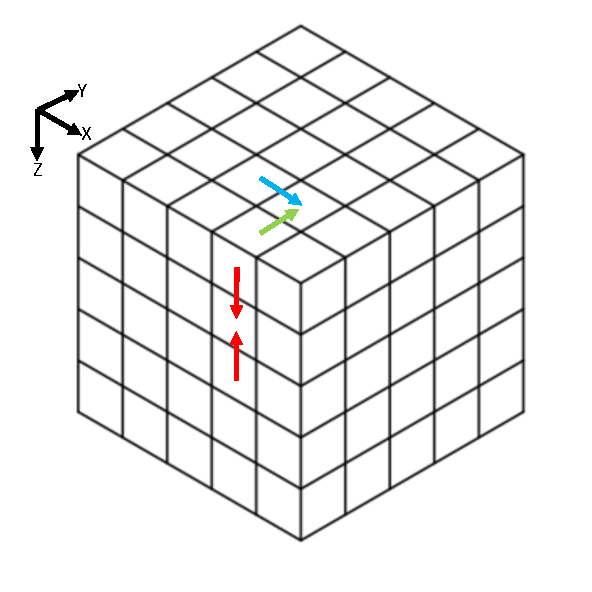
\includegraphics[width=0.8\textwidth]{Fig/demo}
\caption{\wen{PEF direction for a 3D dataset. The two red arrows denote the two-sided prediction in the time axis. Green and blue arrows denote the one-sided prediction along two space axes. All the spatial predictions are one-sided.}}
\label{fig:demo}
\end{figure}



\begin{figure}[htb!]
    \centering
    \subfloat[]{\includegraphics[width=0.45\textwidth]{linear5dn/Fig/synth_clean5d}
    \label{fig:l_clean5d}}
    \subfloat[]{\includegraphics[width=0.45\textwidth]{linear5dn/Fig/synth_obs5d}
    \label{fig:l_obs5d}}\\
    \subfloat[]{\includegraphics[width=0.45\textwidth]{linear5dn/Fig/synth_drr5d}
    \label{fig:l_drr5d}}
    \subfloat[]{\includegraphics[width=0.45\textwidth]{linear5dn/Fig/synth_recon5d}
    \label{fig:l_npef5d}}\\
	\caption{Interpolation results of the noise-free linear-events example for $X=1$ and $Y=1$. (a) Clean data. (b) Decimated data \dlo{by}\wen{with} irregularly missing 70\% traces (S/N=-0.29 dB). (c) Reconstructed data using the rank-reduction method (S/N=30.34 dB). (d) Reconstructed data using the NPEF method (S/N=15.69 dB). }
	\label{fig:l_clean5d,l_obs5d,l_drr5d,l_npef5d}
\end{figure}

\begin{figure}[htb!]
    \centering
    \subfloat[]{\includegraphics[width=0.45\textwidth]{linear5dn/Fig/synth_clean5d-fk}
    \label{fig:l_clean5d-fk}}
    \subfloat[]{\includegraphics[width=0.45\textwidth]{linear5dn/Fig/synth_obs5d-fk}
    \label{fig:l_obs5d-fk}}\\
    \subfloat[]{\includegraphics[width=0.45\textwidth]{linear5dn/Fig/synth_drr5d-fk}
    \label{fig:l_drr5d-fk}}
    \subfloat[]{\includegraphics[width=0.45\textwidth]{linear5dn/Fig/synth_recon5d-fk}
    \label{fig:l_npef5d-fk}}\\
	\caption{\wen{FK spectra of interpolation results of the noise-free linear-events example for $X=1$ and $Y=1$. (a) Clean data. (b) Decimated data. (c) Reconstructed data using the rank-reduction method. (d) Reconstructed data using the NPEF method.} }
	\label{fig:l_clean5d-fk,l_obs5d-fk,l_drr5d-fk,l_npef5d-fk}
\end{figure}

\begin{figure}[htb!]
    \centering
    \subfloat[]{\includegraphics[width=0.35\textwidth]{linear5dn/Fig/synth_apef5-s1}
    \label{fig:l_npef1}}
    \subfloat[]{\includegraphics[width=0.35\textwidth]{linear5dn/Fig/synth_apef5-s2}
    \label{fig:l_npef}}\\
    \subfloat[]{\includegraphics[width=0.35\textwidth]{linear5dn/Fig/synth_apef5-s3}
    \label{fig:l_npef3}}
    \subfloat[]{\includegraphics[width=0.35\textwidth]{linear5dn/Fig/synth_apef5-s4}
    \label{fig:l_npef4}}\\
	\caption{Coefficients cubes of the estimated NPEF for $X=1$ and $Y=1$.  NPEF coefficients corresponding to the first (a), second (b), third (c), and fourth (d) temporal filter indices.   }
	\label{fig:l_npef1,l_npef2,l_npef3,l_npef4}
\end{figure}

\begin{figure}[htb!]
    \centering
    \subfloat[]{\includegraphics[width=0.45\textwidth]{linear5dn/Fig/synth_clean5d-2}
    \label{fig:l_clean5d2}}
    \subfloat[]{\includegraphics[width=0.45\textwidth]{linear5dn/Fig/synth_obs5d-2}
    \label{fig:l_obs5d2}}\\
    \subfloat[]{\includegraphics[width=0.45\textwidth]{linear5dn/Fig/synth_drr5d-2}
    \label{fig:l_drr5d2}}
    \subfloat[]{\includegraphics[width=0.45\textwidth]{linear5dn/Fig/synth_recon5d-2}
    \label{fig:l_npef5d2}}\\
	\caption{Interpolation results of the noise-free linear-events example for $Hx=6$ and $Hy=6$. Each common offset cube has been reshaped into a 2D matrix. (a) Clean data. (b) Decimated data \dlo{by}\wen{with} irregularly missing 70\% traces (S/N=-0.29 dB). (c) Reconstructed data using the rank-reduction method (S/N=30.34 dB). (d) Reconstructed data using the NPEF method (S/N=15.69 dB). }
	\label{fig:l_clean5d2,l_obs5d2,l_drr5d2,l_npef5d2}
\end{figure}


%% The following was reviewed during revision but actually very informative
%\begin{figure}[htb!]
%   \centering
%   \subfloat[]{\includegraphics[width=0.45\textwidth]{linear5dn/Fig/synth_noisy5d}
%   \label{fig:ln_noisy5d}}
%   \subfloat[]{\includegraphics[width=0.45\textwidth]{linear5dn/Fig/nsynth_obs5d}
%   \label{fig:ln_obs5d}}\\
%   \subfloat[]{\includegraphics[width=0.45\textwidth]{linear5dn/Fig/nsynth_drr5d}
%   \label{fig:ln_drr5d}}
%   \subfloat[]{\includegraphics[width=0.45\textwidth]{linear5dn/Fig/nsynth_recon5d}
%   \label{fig:ln_npef5d}}\\
%\caption{Interpolation results of the noisy linear-events example for $X=1$ and $Y=1$. Each common midpoint cube has bee reshaped into a 2D matrix. (a) Noisy data (S/N=-0.66 dB). (b) Decimated data \dlo{by}\wen{with} irregularly missing 70\% traces (S/N=-0.21 dB). (c) Reconstructed data using the rank-reduction method (S/N=16.83 dB). (d) Reconstructed data using the NPEF method (S/N=2.93 dB). Note that the NPEF method fails in this case.}
%\label{fig:ln_noisy5d,ln_obs5d,ln_drr5d,ln_npef5d}
%\end{figure}
%
%\begin{figure}[htb!]
%   \centering
%   \subfloat[]{\includegraphics[width=0.45\textwidth]{linear5dn/Fig/synth_noisy5d-2}
%   \label{fig:ln_noisy5d2}}
%   \subfloat[]{\includegraphics[width=0.45\textwidth]{linear5dn/Fig/nsynth_obs5d-2}
%   \label{fig:ln_obs5d2}}\\
%   \subfloat[]{\includegraphics[width=0.45\textwidth]{linear5dn/Fig/nsynth_drr5d-2}
%   \label{fig:ln_rr5d2}}
%   \subfloat[]{\includegraphics[width=0.45\textwidth]{linear5dn/Fig/nsynth_recon5d-2}
%   \label{fig:ln_npef5d2}}\\
%\caption{Interpolation results of the noisy linear-events example for $Hx=6$ and $Hy=6$. Each common offset cube has bee reshaped into a 2D matrix. (a) Noisy data. (b) Decimated data \dlo{by}\wen{with} irregularly missing 70\% traces. (c) Reconstructed data using the rank-reduction method. (d) Reconstructed data using the NPEF method. Note that the NPEF method fails in this case.}
%\label{fig:ln_noisy5d2,ln_obs5d2,ln_drr5d2,ln_npef5d2}
%\end{figure}
%% The above was reviewed during revision but actually very informative

\begin{figure}[htb!]
   \centering
   \subfloat[]{\includegraphics[width=\textwidth]{linear5da/Fig/la_obs5d-3}
   \label{fig:la_obs5d}}\\
   \subfloat[]{\includegraphics[width=\textwidth]{linear5da/Fig/la_drr5d-3}
   \label{fig:la_drr5d}}\\
   \subfloat[]{\includegraphics[width=\textwidth]{linear5da/Fig/la_recon5d-3}
   \label{fig:la_npef5d}}\\
\caption{De-aliased interpolation results of the linear-events example for $X=3$ and $Y=3$. Each common midpoint cube has bee reshaped into a 2D matrix. (a) Regularly missing data. (b) Reconstructed data using the rank-reduction method. (c) Reconstructed data using the NPEF method. Note that the standard rank-reduction method completely fails in this case.}
\label{fig:la_obs5d,la_drr5d,la_npef5d}
\end{figure}

\begin{figure}[htb!]
   \centering
   \subfloat[]{\includegraphics[width=\textwidth]{linear5da/Fig/la_obs5d-3fk}
   \label{fig:la_obs5dfk}}\\
   \subfloat[]{\includegraphics[width=\textwidth]{linear5da/Fig/la_drr5d-3fk}
   \label{fig:la_drr5dfk}}\\
   \subfloat[]{\includegraphics[width=\textwidth]{linear5da/Fig/la_recon5d-3fk}
   \label{fig:la_npef5dfk}}\\
\caption{\wen{FK spectra of de-aliased interpolation results of the linear-events example for $X=3$ and $Y=3$. Each common midpoint cube has bee reshaped into a 2D matrix. (a) Regularly missing data. (b) Reconstructed data using the rank-reduction method. (c) Reconstructed data using the NPEF method.}}
\label{fig:la_obs5dfk,la_drr5dfk,la_npef5dfk}
\end{figure}

\begin{figure}[htb!]
   \centering
   \subfloat[]{\includegraphics[width=\textwidth]{hyper5da/Fig/ha_obs5d-3}
   \label{fig:ha_obs5d}}\\
   \subfloat[]{\includegraphics[width=\textwidth]{hyper5da/Fig/ha_drr5d-3}
   \label{fig:ha_drr5d}}\\
   \subfloat[]{\includegraphics[width=\textwidth]{hyper5da/Fig/ha_recon5d-3}
   \label{fig:ha_npef5d}}\\
\caption{De-aliased interpolation results of the hyperbolic-events example for $X=3$ and $Y=3$. Each common midpoint cube has bee reshaped into a 2D matrix. (a) Regularly missing data. (b) Reconstructed data using the rank-reduction method. (c) Reconstructed data using the NPEF method. Note that the standard rank-reduction method completely fails in this case.}
\label{fig:ha_obs5d,ha_drr5d,ha_npef5d}
\end{figure}


\begin{figure}[htb!]
   \centering
   \subfloat[]{\includegraphics[width=0.9\textwidth]{real5d/Fig/r_obs5d-3-0}
   \label{fig:r_obs5d}}\\
   \subfloat[]{\includegraphics[width=0.9\textwidth]{real5d/Fig/r_drr5d-3-0}
   \label{fig:r_drr5d}}\\
   \subfloat[]{\includegraphics[width=0.9\textwidth]{real5d/Fig/r_npef5d-3-0}
   \label{fig:r_npef5d}}\\
\caption{Interpolation results of a real 5D seismic data example for $Hx=6$ and $Hy=6$. Each common offset cube has bee reshaped into a 2D matrix. (a) The raw data gridded onto regular grids. Those blank areas denote missing traces. (b) Reconstructed data using the damped rank-reduction method. (c) Reconstructed data using the NPEF method. Note that the damped rank-reduction outperforms the NPEF method in the case of irregularly missing traces.}
\label{fig:r_obs5d,r_drr5d,r_npef5d}
\end{figure}

\begin{figure}[htb!]
   \centering
   \subfloat[]{\includegraphics[width=0.4\textwidth]{real5d/Fig/r_obs5d-cog-zA}
   \label{fig:r_obs5d1a}}
   \subfloat[]{\includegraphics[width=0.4\textwidth]{real5d/Fig/r_obs5d-cog-zB}
   \label{fig:r_obs5d1b}}\\
   \subfloat[]{\includegraphics[width=0.4\textwidth]{real5d/Fig/r_drr5d-cog-zA}
   \label{fig:r_drr5d1a}}
   \subfloat[]{\includegraphics[width=0.4\textwidth]{real5d/Fig/r_drr5d-cog-zB}
   \label{fig:r_drr5d1b}}\\
   \subfloat[]{\includegraphics[width=0.4\textwidth]{real5d/Fig/r_npef5d-cog-zA}
   \label{fig:r_npef5d1a}}
   \subfloat[]{\includegraphics[width=0.4\textwidth]{real5d/Fig/r_npef5d-cog-zB}
   \label{fig:r_npef5d1b}}\\
\caption{Left column: zoomed comparison of frame boxes A in Figure \ref{fig:r_obs5d,r_drr5d,r_npef5d}. Right column: zoomed comparison of frame boxes B in Figure \ref{fig:r_obs5d,r_drr5d,r_npef5d}. Note the strong residual noise seen in (f) caused by the NPEF method. }
\label{fig:r_obs5d1a,r_obs5d1b,r_drr5d1a,r_drr5d1b,r_npef5d1a,r_npef5d1b}
\end{figure}




\begin{figure}[htb!]
   \centering
   \subfloat[]{\includegraphics[width=0.9\textwidth]{real5d/Fig/r_obs5d-4-0}
   \label{fig:r_obs5d4}}\\
   \subfloat[]{\includegraphics[width=0.9\textwidth]{real5d/Fig/r_drr5d-4-0}
   \label{fig:r_drr5d4}}\\
   \subfloat[]{\includegraphics[width=0.9\textwidth]{real5d/Fig/r_npef5d-4-0}
   \label{fig:r_npef5d4}}\\
\caption{Interpolation results of a real 5D seismic data example for $Hx=6$ and $Hy=6$. Each common offset cube has bee reshaped into a 2D matrix. (a) The raw data gridded onto regular grids. Those blank areas denote missing traces. (b) Reconstructed data using the rank-reduction method. (c) Reconstructed data using the NPEF method. Note that the damped rank-reduction outperforms the NPEF method in the case of irregularly missing traces.}
\label{fig:r_obs5d4,r_drr5d4,r_npef5d4}
\end{figure}



\begin{figure}[htb!]
   \centering
   \subfloat[]{\includegraphics[width=0.4\textwidth]{real5d/Fig/r_obs5d-cmg-zA}
   \label{fig:r_obs5d2a}}
   \subfloat[]{\includegraphics[width=0.4\textwidth]{real5d/Fig/r_obs5d-cmg-zB}
   \label{fig:r_obs5d2b}}\\
   \subfloat[]{\includegraphics[width=0.4\textwidth]{real5d/Fig/r_drr5d-cmg-zA}
   \label{fig:r_drr5d2a}}
   \subfloat[]{\includegraphics[width=0.4\textwidth]{real5d/Fig/r_drr5d-cmg-zB}
   \label{fig:r_drr5d2b}}\\
   \subfloat[]{\includegraphics[width=0.4\textwidth]{real5d/Fig/r_npef5d-cmg-zA}
   \label{fig:r_npef5d2a}}
   \subfloat[]{\includegraphics[width=0.4\textwidth]{real5d/Fig/r_npef5d-cmg-zB}
   \label{fig:r_npef5d2b}}\\
\caption{Left column: zoomed comparison of frame boxes A in Figure \ref{fig:r_obs5d4,r_drr5d4,r_npef5d4}. Right column: zoomed comparison of frame boxes B in Figure \ref{fig:r_obs5d4,r_drr5d4,r_npef5d4}. Note the obviously more discontinuous events in (e) and (f) caused by the NPEF method.}
\label{fig:r_obs5d2a,r_obs5d2b,r_drr5d2a,r_drr5d2b,r_npef5d2a,r_npef5d2b}
\end{figure}


\begin{figure}[htb!]
   \centering
  \subfloat[]{\includegraphics[width=1.0\textwidth]{real5d/Fig/r_obs5d_new-3-0}
%    \subfloat[]{\includegraphics[width=1.0\textwidth]{Fig/test2} %eps2pdf problem
   \label{fig:ra_obs5d}}\\
   \subfloat[]{\includegraphics[width=1.0\textwidth]{real5d/Fig/r_npef5d_new-3-0}
   \label{fig:ra_npef5d}}\\
\caption{De-aliased interpolation results of the real 5D seismic data example for $Hx=6$ and $Hy=6$. We treat the reconstructed data using the damped rank-reduction method as the starting data and further interpolate a trace every other traces in the $X$ and $Y$ directions. Each common offset cube has bee reshaped into a 2D matrix. (a) The regularly sampled data. Those blank areas denote missing traces. (b) Reconstructed data using the NPEF method. In this case of regularly missing traces, the rank-reduction method completely fails so we omit its result.}
\label{fig:ra_obs5d,ra_npef5d}
\end{figure}

\begin{figure}[htb!]
   \centering
%    \subfloat[]{\includegraphics[width=1.0\textwidth]{real5d/Fig/r_obs5d_new-3-0}
   \subfloat[]{\includegraphics[width=1.0\textwidth]{real5d/Fig/r_obs5d_new-3fk} %eps2pdf problem
   \label{fig:ra_obs5d_new-3fk}}\\
   \subfloat[]{\includegraphics[width=1.0\textwidth]{real5d/Fig/r_npef5d_new-3fk}
   \label{fig:ra_npef5d_new-3fk}}\\
\caption{\wen{FK spectra of de-aliased interpolation results of the real 5D seismic data example for $Hx=6$ and $Hy=6$. (a) The regularly sampled data before interpolation. (b) Reconstructed data using the NPEF method. }}
\label{fig:ra_obs5d_new-3fk,ra_npef5d_new-3fk}
\end{figure}

\begin{figure}[htb!]
   \centering
   \subfloat[]{\includegraphics[width=0.45\textwidth]{real5d/Fig/r_obs5d_new-cog-zA}
   \label{fig:r_obs5da}}
   \subfloat[]{\includegraphics[width=0.45\textwidth]{real5d/Fig/r_obs5d_new-cog-zB}
   \label{fig:r_npef5db}}\\
   \subfloat[]{\includegraphics[width=0.45\textwidth]{real5d/Fig/r_npef5d_new-cog-zA}
   \label{fig:r_obs5da}}
   \subfloat[]{\includegraphics[width=0.45\textwidth]{real5d/Fig/r_npef5d_new-cog-zB}
   \label{fig:r_npef5db}}\\
\caption{Left column: zoomed comparison of frame boxes A in Figure \ref{fig:ra_obs5d,ra_npef5d}. Right column: zoomed comparison of frame boxes B in Figure \ref{fig:ra_obs5d,ra_npef5d}.}
\label{fig:ra_obs5da,ra_npef5da,ra_obs5db,ra_npef5db}
\end{figure}

\begin{figure}[htb!]
  \centering
  \subfloat[]{\includegraphics[width=\textwidth]{real5dos/Fig/os_obs}
  \label{fig:os_obs}}\\
  \subfloat[]{\includegraphics[width=\textwidth]{real5dos/Fig/os_recon}
  \label{fig:os_recon}}\\
  \subfloat[]{\includegraphics[width=\textwidth]{real5dos/Fig/ts_recon}
  \label{fig:ts_recon}}
\caption{\new{Comparison between the two-step and one-step interpolation strategies. (a) Observed data when binned onto the regular grids of two times denser. (b) Reconstructed data by the one-step rank-reduction interpolation strategy. (c) Reconstructed data by the two-step rank-reduction and NPEF interpolation strategy.}  }
\label{fig:os_obs,os_recon,ts_recon}
\end{figure}


\begin{figure}[htb!]
   \centering
   \subfloat[]{\includegraphics[width=\textwidth]{real2/Fig/zero2d}
   \label{fig:zero2d}}\\
   \subfloat[]{\includegraphics[width=\textwidth]{real2/Fig/recon2d2}
   \label{fig:recon2d2}}\\
   \subfloat[]{\includegraphics[width=\textwidth]{real2/Fig/recon2d}
   \label{fig:recon2d}}\\
\caption{\new{De-aliased interpolation results of the second field data example for a common shot gather. Each gather has bee reshaped into a 2D matrix. (a) Regularly missing data. (b) Reconstructed data using the rank-reduction method. (c) Reconstructed data using the NPEF method. Note that the rank-reduction method completely fails in this case.}}
\label{fig:zero2d,recon2d2,recon2d}
\end{figure}

\begin{figure}[htb!]
   \centering
   \subfloat[]{\includegraphics[width=\textwidth]{real2/Fig/zerofk2d}
   \label{fig:zerofk2d}}\\
   \subfloat[]{\includegraphics[width=\textwidth]{real2/Fig/reconfk2d2}
   \label{fig:reconfk2d2}}\\
   \subfloat[]{\includegraphics[width=\textwidth]{real2/Fig/reconfk2d}
   \label{fig:reconfk2d}}\\
\caption{\new{FK spectra of de-aliased interpolation results of the second field data example.  Each gather has bee reshaped into a 2D matrix. (a) Regularly missing data. (b) Reconstructed data using the rank-reduction method. (c) Reconstructed data using the NPEF method.}}
\label{fig:zerofk2d,reconfk2d2,reconfk2d}
\end{figure}
}

\section{Discussion}
The anti-aliasing ability of the proposed method could be attributed to the time-space domain implementation of the PEF. Since in time-space domain, multi-scale/frequency components are coupled together, thus it is easier to extract the coherency among the datasets. In the frequency domain, however, the seismic data are separated into different frequencies, causing the problem that low-frequency components are more anti-aliasing while the high-frequency components tend to be aliasing. Traditionally, the anti-aliasing effect of the frequency-space domain interpolation method is achieved by constraining the high-frequency solution via the non-aliased low-frequency solution \cite[]{herrmann2000aliased}. \cite{cary2011aliasing}, however, finds that the low-frequency constraint may not be strong enough to enable the anti-aliasing effect for high-frequency components, which results in a poorly reconstructed data volume that mixes the aliased and non-aliased data. \cite{chiu20135d} develop a 5D anti-aliasing minimum weighted norm interpolation (MWNI) method by a two-step strategy. In the first step, an approximate initial model is obtained. In the second step, the initial model is used to compute the spectral weights to constrain the least-squares solutions of MWNI. Although the method was found to be effective, it is less straightforward and the performance highly depends on initial model. The proposed method, due to its time-domain implementation, is more convenient to conquer the aliasing issue.

Although mathematically the proposed NPEF method is similar to the slope estimation method based on PWD, it does not suffer from the high-frequency limitation as the PWD method.  The reason why PWD method suffers from the high-frequency limit is that one needs to seek an explicit approximation of the phase-shift operator via a third-order and fifth-order filter (as a function of the local slope $\sigma$), e.g., in equations 12 or 13. Only if we have an explicit relation between the phase-shift operator and the local slope $\sigma$ can we use non-linear inversion methods to solve for the local slope. However, the accuracy of the approximation is greatly decreased for high frequencies, as illustrated by Figure 1 in \cite{fomel2002pwd}. However, in the NPEF method introduced here, the local slope is implicitly involved in the prediction filter coefficients $C_{n_t,n_x}(t,x)$. The large approximation error in high frequencies no longer exists.%In other words, in NPEF, we do not care the slope, only care the filter coefficients of PWD.}

We solve the NPEF coefficients due to the convenience and capabilities of the shaping regularization method. It is widely known that the standard L2 norm applied onto the solution is a type of smooth regularization, which, in this regard, is similar to the shaping regularization method. Compared with the shaping regularization, the L2 norm constraint is a global regularization (or global smoothing). The L2 norm regularized inverse problem is usually solved via a damped least-squares method. The damping has the effect of smoothing. Normally, the damping is globally consistent. But via shaping regularization, one can apply a smoothing filter to the solution, which is a local operation. Thus, the shaping regularization better preserves the local features (or resolution) of the solution.

Several synthetic and field datasets show that the NPEF method can be an effective method for interpolating both irregularly sampled data or the more challenging regularly sampled data. Although it is capable of interpolating the irregularly missing traces especially when the S/N is relatively high, it is recommended to be combined with a more advanced interpolation method for irregularly missing traces, e.g., the freely available rank-reduction method ($http://ahay.org/RSF/book/tccs/drr5d/paper\_html/$). The rank-reduction method, however, is less competent in densifying the spatial sampling. In the current interpolation framework, it does not work effectively for very noisy data due to the hard constraint in the interpolation model in equation \ref{eq:inv44}, which means that the existing noisy traces are directly used as the output traces. It is worth investigating an anti-noise strategy by modifying equation \ref{eq:inv44} in the NPEF interpolation framework in the future research.  


\section{Conclusions}
We have extended the PEF from common 2D/3D applications to a 5D problem, i.e., 5D seismic data interpolation. The NPEF is the non-stationary version of the PEF filter, where the coefficients of a fixed-size PEF vary with the time and space locations. The NPEF is in a 10D space where the first five dimensions correspond to the filter coefficients for a specific point in the 5D data space. To solve the highly ill-posed inverse problem that involves the 10D NPEF, we use the \new{computationally efficient} shaping regularization method, where the solution is constrained to be smooth with \old{an efficient 5D}\new{a} triangle smoothing operator. To interpolate the missing traces, another inverse problem needs to be solved, where the solution is constrained by the 10D NPEF. The performance of the proposed NPEF method is tested by two synthetic and a real seismic dataset, in the cases of both irregularly sampled and regularly sampled traces, and benchmarked with the state-of-the-art rank-reduction method. Results show that the proposed method outperforms the rank-reduction method in interpolating regularly sampled seismic data although \dlo{being}\wen{is} less effective in reconstructing the irregularly missing traces \new{especially in the presence of strong random noise}.

\section{DATA AND MATERIALS AVAILABILITY}
Data associated with this research are available and can be obtained by contacting the corresponding author.

\bibliographystyle{seg}
\bibliography{npef}


\newpage
\listoffigures




